\documentclass[a4paper]{report}

\usepackage[english]{babel}
\usepackage[utf8]{inputenc}
\usepackage{geometry}
\usepackage{amsthm}
\usepackage{amsmath}
\usepackage{amssymb}
\usepackage{mathrsfs}
\usepackage{enumerate}

\usepackage{tikz}
\usetikzlibrary{positioning}
\usepackage{tikz-cd}

\newcommand{\RE}{\mathrm{Re}}
\newcommand{\IM}{\mathrm{Im}}
\newcommand{\function}[5]{\begin{array}{l|rcl}
#1: & #2 & \longrightarrow & #3 \\
    & #4 & \longmapsto & #5 \end{array}}
\newtheorem{theorem}{Theorem}[section]

\title{AAQDD -- Abstract additive quantum decision diagrams}
\author{M. Leroy, R. Vilmart}

\begin{document}

\maketitle

\tableofcontents

\newpage

\chapter{Complex intervals arithmetics}

\section{Generalities}

The purpose of quantum decision diagrams is to provide a more efficient way to store and manipulate quantum states of a finite number of qubits. A $n$-qubit state is indeed traditionally represented as an element of $\mathbb{C}^{2^n}$ (with norm 1), which takes exponential space as $n$ grows. Abstract states will be in this part defined similarly, but with complex intervals instead of complex numbers.

\subsection{Real intervals}

The standard definition of real intervals is:
$$\forall a, b \in \mathbb{R}, [a, b]
= \{x \in \mathbb{R} / \min(a, b) \le x \le \max(a, b)\}$$

From now on, the set of real intervals will be noted $\mathcal{A}_0(\mathbb{R})$. Of course, $\mathcal{A}_0(\mathbb{R}) \subset \mathcal{P}(\mathbb{R}) \subset \mathcal{P}(\mathbb{C})$. While not being sufficient to handle completely our operations on quantum states, caracterized by complex amplitudes, these real intervals will still be useful. Moreover, they are well-known and many papers already studied them.

\subsection{Closure \& operations}
\label{closure-operations}

Let $E \subset \mathcal{P}(\mathbb{C})$ a set containing sets of $\mathbb{C}$ (later on, our intervals).

\begin{definition}[closure]
    The closure $\mathscr{C}$ of a set $a \in \mathcal P (\mathbb C)$ is defined by

    $$\mathscr{C}(a) = \bigcap_{\gamma \supset a \mand \gamma \in \mathcal{A}_0(\mathbb{C})} \gamma$$

    Additionally, for any operator
    $\odot : {\mathcal{A}_0}^2 \rightarrow \mathcal{P}(\mathbb C)$,
    we define the operator
    $\mathscr C(\odot) : {\mathcal{A}_0}^2 \rightarrow \mathcal{A}_0$
    such that
    $$\forall a, b \in \mathcal P (\mathbb C),
    a ~ \mathscr C(\odot) ~ b = \mathscr C (a \odot b)$$
\end{definition}

\begin{prop}[colsure]
    The closure is well-defined.
    \begin{itemize}
        \item If $\odot$ is commutative, so is $\cdot$
        \item 
    \end{itemize}
\end{prop}

\begin{definition}[operations]
    Let $E \subset \mathcal{P}(\mathcal C)$. We define for $\alpha, \beta \in \mathcal{P}(\mathbb C)$ the following operations
    $$\alpha \otimes \beta = \{a b ; a \in \alpha, b \in \beta\}$$
    $$\alpha \oplus \beta = \{a + b ; a \in \alpha, b \in \beta\}$$

    Note that none of these sets are in $E$ in the general case, despite it being the case for $E = \mathcal{A}_0(\mathbb{R})$. We define the \textbf{sum} in $\mathcal{A}_0$ to be $+ = \mathscr{C}(\oplus)$ and the \textbf{product} in $\mathcal{A}_0$ to be $\cdot = \mathscr{C}(\oplus)$. Additionally, we define the \textbf{join} $\sqcup = \mathscr{C}(\cup)$.
\end{definition}

\noindent Remarkably, in + is the same as $\oplus$ and $\cdot$ is the same as $\otimes$. On complex intervals, we will see later that this is not necessarily the case.

\begin{definition}[modulus]
    For all $\alpha$ in $E$, we define when it exists
   $\forall \alpha \in E, |\alpha| = \sup\{|a| ; a \in \alpha\}$.
\end{definition}

This general case on a contextual set $E$ leads to defining a \textbf{partial order $\le$}, which really is the subset relation $\supset$, but implying that the sets are all intervals of the same interval set $E$. We easily get the following properties
\begin{enumerate}[i]
    \item $\forall \alpha_1, \beta_1, \alpha_2, \beta_2 \in \mathcal{A}_0, \alpha_1 \le \alpha_2 ~\text{and}~ \beta_1 \le \beta_2 \Rightarrow \alpha_1 + \alpha_2 \le \beta_1 + \beta_2$
    \item $\forall \alpha_1, \beta_1, \alpha_2, \beta_2 \in \mathcal{A}_0, \alpha_1 \le \alpha_2 ~\text{and}~ \beta_1 \le \beta_2 \Rightarrow \alpha_1 \alpha_2 \le \beta_1 \beta_2$
\end{enumerate}

Note that in the case of $\mathcal{A}_0(\mathbb{R})$, the sum and product are \textbf{direct}, meaning that for all $\alpha, \beta \in \mathcal{A}_0^+, \alpha + \beta = \alpha \oplus \beta$ and $\alpha \beta = \alpha \otimes \beta$. To prove that the sum (respectively, the product) is direct, it is enough to prove that summing (respectively multiplying) two elements of $E$ yields another element of $E$.

The operations $\oplus, \otimes, \sqcup, +$ and $\cdot$ are obviously commutative, but only $\oplus$ and $\otimes$ are always associative no matter the set $E$. Proving the directness of the sum or the product in $E$ is hence a way to prove their associativity in $E$.

\subsection{Remarkable subsets}

Intervals of $\mathcal{A}_0(\mathbb{R})$, while being already unsifficient to fully cover the use of intervals in a quantum context, contain even more resricted subsets that will be useful in the next sections. The set of positive intervals $\mathcal{A}_0^+ = \mathcal{A}_0(\mathbb{R}) \cap \mathcal{P}(\mathbb{R})$ is remarkably convenient because it is working well with the operations defined above.

First, $\mathcal{A}_0^+$ is stable for +, $\cdot$ and $\sqcup$, meaning that using these operations on two elements of $\mathcal{A}_0^+$ results in another element of $\mathcal{A}_0^+$. Second, for all real number $0 \le a_1 \le b_1$ and $0 \le a_2 \le b_2$
$$[a_1, b_1] + [a_2, b_2] = [a_1 + a_2, b_1 + b_2]$$
$$[a_1, b_1] [a_2, b_2] = [a_1 a_2, b_1 b_2]$$

Let $\mathcal{A}_0^{2\pi} = \mathcal{A}_0^+ \cap \mathcal{P}([0, 2\pi])$. While $\mathcal{A}_0^{2\pi}$ is not stable, it will be useful in section \ref{polar}.

\begin{theorem}[intervals of the exponential]
Let $\theta \in \mathcal{A}_0^+$, there is a unique $\varphi \in \mathcal{A}_0^{2\pi}$ such that
$$\exp(i\theta) = \exp(i \varphi)$$
\end{theorem}

\begin{proof}
There are unique $\theta^-, \theta^+, \mathbb{R}^+$ such that $\theta = [\theta^-, \theta^+]$ and $\theta^- \le \theta^+$.
% TODO: change the definition?

\end{proof}


\section{Cartesian intervals}

\subsection{Definition}

Real intervals can be generalised to complex intervals naturally using the cartesian notation of complex numbers.
$$\forall x, y \in \mathbb{C}, [x, y]
= \{a + ib ; a \in [\RE(x), \RE(y)], b \in [\IM(x), \IM(y)]\}$$

Similarly to what can be done with real intervals, we can see complex numbers as complex intervals that only have one element, hence we might use $\mathbb{C}$ to be $\{[z, z] ; z \in \mathbb{C}\}$. Now let $\mathcal{A}_0 = \{[x, y] ; x, y \in \mathbb{C}\}$.

\subsection{Operations}

The basic operations on $\mathcal{A}_0$ (sum, product and join) are defined thanks to subsection \ref{general-operations}. Note that the product is \underline{not} associative in $\mathcal{A}_0$, and that the sum is \underline{not} distributive on the product:
$$\forall \alpha, \beta, \gamma \in \mathcal{A}_0, (\alpha + \beta) \gamma \subset \alpha \gamma + \beta \gamma$$

\noindent \underline{\textbf{Proof:}}
\begin{align*}
(\alpha + \beta)\gamma &= \{xc ; x \in \{a + b ; a \in \alpha, b \in \beta\}, c \in \gamma\} \quad \text{(by definition of the product)}\\
&= \{(a + b)c ; a \in \alpha, b \in \beta, c \in \gamma\} \\
&= \{ac + bc ; a \in \alpha, b \in \beta, c \in \gamma\} \\
&\subset \{ac + bd ; a \in \alpha, b \in \beta, c, d \in \gamma\} \\
&\subset \{ac; a \in \alpha, c \in \gamma\} + \{bc ; b \in \beta, c \in \gamma\} \quad \text{(by definition of the sum)} \\
&\subset \alpha \gamma + \beta \gamma
\end{align*}
\hfill{} $\boxed{}$

\subsection{Convex conservation}

All complex intervals are convex.

\noindent \underline{\textbf{Proof:}} Let $\alpha \in \mathcal{A}_0$ and $a, b \in \alpha$. Additionally let $t \in [0, 1]$.

\begin{align*}
\RE(ta+(1-t)b) &= \RE(ta) + \RE((1-t)b) \\
&\le t\RE(a) + (1-t)\RE(b) \quad (\text{since}~t, 1-t \in \mathbb{R}) \\
&\le \max(\RE(\alpha)) \quad \text{since}~a, b \in \alpha
\end{align*}

The corresponding properties with a minimum or the imaginary part are proven very similarly, hence $ta+(1-t)b \in \alpha$.
\hfill{} $\boxed{}$

\subsection{The minus operation}

This gives \textit{almost} us an ring structure for $(\mathcal{A}_0, +, \cdot)$, which we will use just next, and form now on we will note $0 = [0, 0]$ and $1 = [1, 1]$. However it is indeed not a ring because $(\mathcal{A}_0, +)$ is not a group. In fact, the exitence of an opposite (additive inverse) in $\mathcal{A}_0$ is replaced by the following property, which implies that almost no complex interval has an opposite:
$$\forall \alpha,\beta \in \mathcal{A}_0, \alpha \not\in \mathbb{C} \Rightarrow \alpha + \beta \not= 0$$

\noindent \underline{\textbf{Proof:}} Let $\alpha, \beta \in \mathcal{A}_0$, such that $\alpha \not\in \mathbb{C}$. Let $b \in \beta$.
Now, since $\alpha \not\in \mathbb{C}$ there are at least two different complex numbers $x, y \in \mathbb{C}$ in $\alpha$. Hence one of them $z \in \{x, y\}$ is different from $-b$, so $z + b \in \alpha + \beta ~\text{and}~ z + b \not=0$ and finally $\alpha + \beta \not= 0$.
\hfill{} $\boxed{}$

\vspace{1em}
This implies the non-existence of an additive inverse for all non-constant intervals, which breaks any ring structure we could try to build on $+$. Despite that, we can still define a minus operation
$$\forall \beta \in \mathcal{A}_0, -\beta = \{-b ; b \in \beta\}$$
$$\forall \alpha, \beta \in \mathcal{A}_0, \alpha - \beta = \alpha + (- \beta)$$

What is important keep in mind is that we cannot do things like "$\alpha + \beta = \gamma$ \textit{so} $\alpha = \gamma - \beta$", for example if $\alpha = \beta = [0, 1]$. Fundamentally, $\alpha - \alpha \not= 0$.

\subsection{Partial order on intervals}

We define the relation $\le$ on $\mathcal{A}_0$ such that $\forall \alpha, \beta \in \mathcal{A}_0, \alpha \le \beta \Rightarrow \alpha \subset \beta$.
We easily get the following properties:
\begin{enumerate}[i]
    \item $\forall \alpha, \beta \in \mathcal{A}_0, \alpha \le \beta \Rightarrow \alpha^c \le \beta^c$
    \item $\forall \alpha, \beta, \gamma \in \mathcal{A}_0, \alpha \gamma \le \beta \gamma ~\text{and}~ \gamma \not=0 \Rightarrow \alpha \le \beta$
\end{enumerate}

\subsection{Centering}

For all $\alpha \in \mathcal{A}_0$, we introduce $\mu(\alpha) \in \mathbb{C}$ the \textit{middle} of $\alpha$:
$$\mu(\alpha) = \frac{\min(\RE~\alpha) + \max(\RE~\alpha)}{2} + i \frac{\min(\IM~\alpha) + \max(\IM~\alpha)}{2}$$
This notion comes with the following properties:
\begin{enumerate}[i]
    \item $\forall x \in \mathbb{C}, \mu([x, x]) = x$
    \item\label{musum} $\forall \alpha, \beta \in \mathcal{A}_0, \mu(\alpha + \beta) = \mu(\alpha) + \mu(\beta)$
    \item \label{muscalarprod}$\forall \alpha \in \mathcal{A}_0, \forall \lambda \in \mathbb{C}, \mu(\lambda \alpha) = \lambda \mu(\alpha)$ and more generally,
    \item $\forall \alpha, \beta \in \mathcal{A}_0, \mu(\alpha \beta) = \mu(\alpha) \mu(\beta)$
\end{enumerate}

\noindent\underline{\textbf{Proofs:}}
\begin{enumerate}[i]
    \item $\RE([x, x]) = \RE(x)$ and $\IM([x, x]) = \IM(x)$, hence the result.
    \item $\forall \alpha, \beta \in \mathcal{A}_0, \RE(\alpha + \beta) = \RE(\alpha) + \RE(\beta)$
    \item The result is obvious for $\lambda \in \mathbb{R}$.
    Moreover it is clear that $\IM(i \alpha) = \RE(\alpha)$ and similarly that $\RE(i \alpha) = - \IM(\alpha)$, thus
    \begin{align*}
        \mu(i\alpha) &= \frac{\min(-\IM~\alpha) + \max(-\IM~\alpha)}{2} + i \frac{\min(\RE~\alpha) + \max(\RE~\alpha)}{2} \\
        &= \frac{(-\max(\IM~\alpha)) + (-\min(\IM~\alpha))}{2} + i \frac{\min(\RE~\alpha) + \max(\RE~\alpha)}{2} \\
        &= - \IM(\mu(\alpha)) + i \RE(\mu(\alpha)) \\
        &= i \mu(\alpha)
    \end{align*}
    Property \ref{musum} enables us to conclude.
    \item The case when $\alpha$ is a real interval is easy. Using property \ref{muscalarprod} and the almost-ring structure of $\mathcal{A}_0$, the general case is proven.
    \hfill{} $\boxed{}$
\end{enumerate}

\noindent From these properties, it follows that $\mu$ is an almost-ring morphism.

For all $z \in \mathbb{C}$, let $\pm z = [-z, z]$ (obviously $\mu(\pm z) = 0$).
\begin{theorem}[central decomposition]
    $$\forall \alpha \in \mathcal{A}_0, \exists z \in \mathbb{C}, \{y \in \mathbb{C} / \alpha = \pm y + \mu(\alpha)\} = \{z, -z, \bar{z}, -\bar z\}$$
\end{theorem}
\begin{proof}
    The existence on real intervals comes easily from the definition of $\mu$.
    Now for $\alpha \in \mathcal{A}_0$, $\alpha = \RE(\alpha) + i~\IM(\alpha)$, hence the existence of $z$ such that $\{z, -z, \bar{z}, -\bar z\} \subset \{y \in \mathbb{C} / \alpha = \pm y + \mu(\alpha)\}$.
    The reciprocal inclusion comes from the fact that, for real numbers, it is true.
\end{proof}

Now let $\alpha^c$ be this centered interval $\alpha - \mu(\alpha)$, and $\mathcal{A}_0^c = \text{Ker}(\mu)$ be the sub-almost-ring of centered intervals. Now that we defined the centered version of an interval, we can come back to computing $\alpha - \alpha$
$$\forall \alpha \in \mathcal{A}_0, \alpha - \alpha = 2(\alpha^c) = (2\alpha)^c$$

\begin{align*}
\alpha - \alpha
&= \mu(\alpha) + \alpha^c + (\mu(-\alpha) + (-\alpha)^c)\\
\end{align*}

\subsection{Magnitude}

For all $\alpha \in \mathcal{A}_0$, we introduce $|\alpha| \in \mathbb{R}$ the \textit{magnitude} of $\alpha$

$$|\alpha| = \max \{|x| ; x \in \alpha\}$$

\begin{prop}[magnitude from boundaries]
    $$\forall x, y \in \mathbb C, \left|[x, y]\right| = \max (|x|, |y|)$$
\end{prop}
\begin{proof}
    Let $x, y \in \mathbb C$. $|x| \in \{|z| ; z \in [x, y]\}$ so $|x| \le \left|[x, y]\right|$ and $|y| \le \left|[x, y]\right|$ thus $\max (|x|, |y|) \le \left|[x, y]\right|$.
    Now let $z \in [x, y]$. $|\RE(z)| \le \max (|\RE(x)|, |\RE(y)|)$ and equally for the imaginary part, hence $|z| \le \max (|x|, |y|)$ by the triangular inequality, so $|[x, y]| \le \max (|x|, |y|)$.
\end{proof}


\section{Polar intervals}
\label{polar}

\subsection{Definition}

We have seen that cartesian complex intervals have interesting properties on sums while being harder to manipulate with products. Given the multiplicative nature of some of the structures we will define in the next chapter, is seems interesting to define a kind of complex interval that works better with products. Polar intervals were defined .

A polar complex interval is $\rho e^{i\theta}$ for $\rho, \theta \in \mathcal{A}_0^+$ (the product between $\rho$ and $e^{i\theta}$ here is $\otimes$). The set of polar complex intervals is $\mathcal{S}_0$.

\subsection{Operations}

The most interesting property of polar complex intervals is the following.

\begin{theorem}[directness of the product]
The product is direct in $\mathcal{S}_0$.
\end{theorem}
\begin{proof}
Let $\rho, \eta, \theta, \varphi \in \mathcal{A}_0^+$. By associativity and commutativity of $\otimes$,
\begin{align*}
    (\rho \otimes e^{i\theta}) \otimes (\eta \otimes e^{i\varphi})
    &= (\rho \eta) \otimes e^{i\theta} \otimes e^{i\varphi} \\
    &= \{r e^{it} e^{ip} ; r \in \rho \otimes \eta, t \in \theta, p \in \varphi\} \\
    &= \{r e^{i(t+p)} ; r \in \rho \otimes \eta, t \in \theta, p \in \varphi\} \\
    &= \{r e^{i(t+p)} ; r \in \rho \otimes \eta, x \in \theta \oplus \varphi\} \\
    &= \{r e^{i(t+p)} ; r \in \rho \eta, x \in \theta + \varphi\} \\
    & \quad \quad (\text{by directness of the sum and product in } \mathcal{A}_0^+) \\
    &= \rho \eta e^{i(\theta + \varphi)} \in \mathcal{S}_0
\end{align*}
\end{proof}



\chapter{States \& diagrams}

\section{Abstract states}

We now have intervals, \textit{abstract elements} of $\mathbb{C}$ represented in $\mathcal{A}_0$. Our abstract elements for a $n$-qubit quantum state would be in $\mathcal{A}_n = {\mathcal{A}_0}^{2^n}$ for all $n \in \mathbb{N}$. Defining a sum in $\mathcal{A}_n$, and an external product $\alpha * A$ for
$\alpha \in \mathcal{A}_0$ and $A \in \mathcal{A}_n$, comes easily. We also define the inclusion relation in $\mathcal{A}_n$ (which is an order relation) $\subset$ using the cartesian product of sets:
$$\forall A = (a_0, ..., a_{2^n-1})^{T},  B = (b_0, ..., b_{2^n-1})^{T} \in \mathcal{A}_n, A \subset B \iff a_0 \times ... \times a_{2^n-1} \subset b_0 \times ... \times b_{2^n-1}$$

Intuitively, if $A$ and $B$ are in $\mathcal{A}_n$ and $A \subset B$, the abstract state $A$ is more \textit{precise} than $B$.

\section{Decision diagrams}

We inductively define abstract additive quantum decision diagrams (AAQDDs), starting from zero-depth decision. The only zero-depth diagram is $\boxed{1}$. Let for every set $E$ be the set of finite subsets of $E$: $\mathscr{P}_f(E) = \{ A \subset E / |A| < \infty \}$. If the set $\mathcal{D}_n$ of diagrams of depth $n$ is defined, $n+1$-depth diagrams can have a finite number of left children in $\mathcal{D}_n$ and a finite number of right children in $\mathcal{D}_n$, each being associated with an abstract amplitude in $\mathcal{A}_0$.

\begin{center}
    % https://tikzcd.yichuanshen.de/#N4Igdg9gJgpgziAXAbVABwnAlgFyxMJZAZgBoAGAXVJADcBDAGwFcYkQAREAX1PU1z5CKcqQCM1Ok1bsoAfXI8+IDNjwEiY8ZIYs2iEADpjS-mqFEATNpq6ZB+cDABaMd1MqB64cgAsNqT12AHM5MQ9VQQ0UAFYAu30jE14zKJ8ANnjpRNDgAFtXd25JGChg+CJQADMAJwg8pFEQHAgkMkD7EAAdLqY0AAt6OSdCkBpGegAjGEYABS8LA0YYKpwxkEYsMESoejh+0o9a+saaFqR-DsSe6ZwhxXGpmfnzaJAarGD+tZSQY4bEE1zohMld2DcYHdhgU3OsJtM5gs3stVkc6gCga1EFowQYen1Bgo4U9Ea9hO9Pt84VsdnsDlAeJRuEA
    \begin{tikzcd}
        &     &         & D \arrow[ld, "\alpha_{n-1}", dashed] \arrow[rd, "\beta_0"'] \arrow[rrrd, "\beta_{m-1}"] \arrow[llld, "\alpha_0"', dashed] &     &     &         \\
    d_0 & ... & d_{n-1} &                                                                                                                           & g_1 & ... & g_{m-1}
    \end{tikzcd}
\end{center}

Defining $\mathcal{D}_{n+1} = \mathscr{P}_f(\mathcal{A}_0 \times \mathcal{D}_n) \times \mathscr{P}_f(\mathcal{A}_0 \times \mathcal{D}_n)$ thus comes naturally. Eventually, let $\mathcal{D} = \bigcup_{n \in \mathbb{N}} \mathcal{D}_n$ the set of all AAQDDs.

\section{Sub-diagrams}

Sub-diagrams (or nodes) of a diagram $D \in \mathcal{D}_n$ for all $n \in \mathbb{N}$, are defined inductively:
$$\mathcal{N}(\boxed{1}) = \boxed{1}$$
$$\forall D, G \in \mathscr{P}_f(\mathcal{A}_0 \times \mathcal{D}_n), \mathcal{N}(D, G) = \{d ; (\alpha, d) \in D \cup G\} \cup
\bigcup_{(\alpha, d) \in D \cup G} \mathcal{N}(d)$$

We also define $\mathcal{N}_i(D) = \mathcal{N}(D) \cap \mathcal{D}_i$ for all $i \in \mathbb{N}$ the nodes "at height $i$".

\section{Diagram evaluation}

Now that we defined our decision diagrams, we can evaluate them to get abstract elements. We inductively define our evaluation function for $n$ quibits $\mathcal{E}_n : \mathcal{D}_n \rightarrow \mathcal{A}_n$:

$$\mathcal{E}_0(\boxed{1}) = \{1\}$$

$$\forall D, G \in \mathscr{P}_f(\mathcal{A}_0 \times \mathcal{D}_n), \mathcal{E}_{n+1}(D, G) =
\begin{pmatrix}
    \displaystyle\sum_{(\alpha, g) \in G} \alpha * \mathcal{E}_n(g) \\
    \displaystyle\sum_{(\beta, d) \in D} \beta * \mathcal{E}_n(d) \\
\end{pmatrix}
\quad\text{with}
$$

Since there is no risk of ambiguity, defining $\mathcal{E} : \bigcup \mathcal{D}_n \rightarrow \bigcup \mathcal{A}_n$ is not problematic. With this last function, we can now evaluate all our AAQDDs and define a partial order $\le$ on $\mathcal{D}$, with:
$$\forall A, B \in \mathcal{D}, A \le B \iff \mathcal{E}(A) \subset \mathcal{E}(B)$$

Additionally, we extend the definition of the imprecision function $\mathcal{I}$ to diagrams: $\forall D \in \mathcal{D}, \mathcal{I}(D) = \mathcal{I}(\mathcal{E}(D))$. Note that $\forall A, B \in \mathcal{D}_n, A \le B$ implies that $\mathcal{I}(A) \le \mathcal{I}(B)$ but that the reciprocal is not generally true.

\section{Error estimation}

Let $A, C \in \mathcal{D}_n$. We would like to define a scale $\delta : \mathcal{D}_n \rightarrow X$ with $(X, \prec)$ a partially ordered set, that we would be able to compute in polynomial time and space (i.e. in $O(n^p)$ for a certain $p \in \mathbb{N}$), such that if $A \le C$, $\delta(A) \prec \delta(C)$. Let $X = \mathbb{R}^+ \times \mathcal{A}_0$ and $\delta(A) = (|A|, [A])$ be inductively defined by:
$$\delta(\boxed{1}) = (1, [1, 1])$$
$$\forall a, b \in \mathcal{A}_0, \delta(\{(a, \boxed{1})\}, \{(b, \boxed{1})\}) = $$
$$\forall G, D \in \mathscr{P}_f(\mathcal{A}_0 \times \mathcal{D}_n), |(G, D)|
= \max\left( \left|\sum_{(l, L) \in G} l |L| \right|, \left|\sum_{(r, R) \in D} r |R| \right|\right)$$
$$\forall G, D \in \mathscr{P}_f(\mathcal{A}_0 \times \mathcal{D}_n), [(G, D)]
= \left(\sum_{(l, L) \in G} l |L| [L] \right) \bigsqcup \left(\sum_{(r, R) \in D} r |R| [R]\right)$$

\noindent\underline{\textbf{Proof:}} Let for $n \ge 0$ the property
$$(\Delta_n)\quad : \quad \forall A, B \in \mathcal{D}_n, A \le B \Rightarrow \delta(A) \prec \delta(B)$$

\noindent\boxed{n = 0} The only zero-height diagram is $\boxed{1}$, the result is trivial.

\noindent\boxed{n = 1} Let $A, B \in \mathcal{D}_1$.

\begin{center}
% https://tikzcd.yichuanshen.de/#N4Igdg9gJgpgziAXAbVABwnAlgFyxMJZABgBpiBdUkANwEMAbAVxiRAEEQBfU9TXfIRQAmclVqMWbAELdeIDNjwEiZAIzj6zVohAAdPQCMIADxhRgarnL5LBRURupapug8bMWr3ceYDm8ESgAGYAThAAtkhkIDgQSKIS2mx0APoMAH4ZINQMdIYwDAAK-MpCIKFYfgAWODkgDFhgOiBQdHDV5vUFYFBIALQALACcPCHhUYgxcQnOki1ZaaH1eQXFpfa6DDDBddQ9fYgjYyBhkUhq1DOIAMxzybqG6Vkr+YUldiq6lTV7DU0tNodLr7GC9AbHeRnSaXWLxW73VwgLJPZa5N7rT7lba7bpgw7HChcIA
\begin{tikzcd}
A \arrow[d, "a_l~~"', dashed, bend right=49] \arrow[d, "~~a_r", bend left=49] &  & B \arrow[d, "b_l~~"', dashed, bend right=49] \arrow[d, "~~b_r", bend left=49] \\
\boxed{1}                                                                     &  & \boxed{1}
\end{tikzcd}
\end{center}

Suppose that $A \le B$, then $a_l \le b_l$ and $a_r \le b_r$, hence $a_l [\boxed{1}] \sqcup a_r [\boxed{1}] = a_l + a_r \le b_l + b_r$, and then $\delta(A) \prec \delta(B)$, so $(\Delta_1)$ is true.

\noindent\boxed{n > 1} Let $n > 1$ such that $(\Delta_{n-1})$ is true. Let $A, B \in \mathcal{D}_n$ such that $A \le B$.

% https://tikzcd.yichuanshen.de/#N4Igdg9gJgpgziAXAbVABwnAlgFyxMJZAJgBoAGAXVJADcBDAGwFcYkQBBEAX1PU1z5CKAKwVqdJq3YAhHnxAZseAkXKkAjBIYs2iEABkA+hvn9lQohs3apew0cK9zg1SjJaaO6foBKJs0UBFWFkAGYbLzt2fwBbQKVXUIAWSMlddmNTZyCLN2QxT3SfBycFRJCiADY073t-bPLgyxQAdlrovyN47gkYKABzeCJQADMAJwh4xHUQHAgkCOK9MGZGRhpGegAjGEYABWa3EEYYUZwQTawweyh6OAALfsCJqaRZ+aRU5aRV9c2dntDnlhCczhccq9ph8FogxD9EH8NidAQcjqDTucXpNoTRPogyAikQDdmiQexMRcrjd2HdHs9ITikNY5rCakS1sitqTgUkKeDLidrrd7k8oNi3ogWfj2hz-iieej+VjqSL6eLGZLpbCABxRDKIzkkoFK-SUiXTbVIACc+p8xIVJvJZoFmumhPxSzqvyNjrJfJdKpAT3o4v0kBpqtpEBwOAZCihXzxsPh3sN8u5ToDYKDIbD4AIbCj+igMbjGoTTMQ7JldpWvsz-sqgapwZgofYEaLQppJbL8bGVb1rJtdZ9GdRvObOdbec7hcFjGF0djDMo3CAA
\begin{tikzcd}
                               &     & A \arrow[ld, dashed] \arrow[d] \arrow[rd] \arrow[lld, dashed] &     &                                & B \arrow[ld, dashed] \arrow[d, dashed] \arrow[rd] \arrow[rrd] &                                &     \\
L_1 \arrow[r, no head, dotted] & L_n & R_1 \arrow[r, no head, dotted]                                & R_m & L_1 \arrow[r, no head, dotted] & L_n                                                           & R_1 \arrow[r, no head, dotted] & R_m
\end{tikzcd}

Let $a_j = \text{ampl}(j, A)$ and $b_j = \text{ampl}(j, B)$. We know that $A \le B$ so:
$$\sum_j a_j \mathcal{E}(j) \le \sum_j b_j \mathcal{E}(j)$$

We would like to prove that:
$$|A \le |B|, ~\text{i.e.}~ \max()$$

\section{Non-additive diagrams}

We can also define non-additive diagrams, which are diagrams that have at most one left child and one right child. We define $\mathcal{D}^* = \bigcup_{n \in \mathbb{N}} \mathcal{D}^*_n$ the set of all non-additive diagrams, with $\mathcal{D}^*_n = \mathscr{S}(\mathcal{A}_0 \times \mathcal{D}^*_{n-1}) \times \mathscr{S}(\mathcal{A}_0 \times \mathcal{D}^*_{n-1})$ and $\mathscr{S}(E) = \{ \{x\} ; x \in E\} \cup \{\emptyset\}$. As we will see in the next chapter, non-additive diagrams have convenient properies that are not generally verified in additive diagrams, enabling us to provide a reduction algorithm.

\begin{wrapfigure}{r}{0pt}
% https://tikzcd.yichuanshen.de/#N4Igdg9gJgpgziAXAbVABwnAlgFyxMJZABgBpiBdUkANwEMAbAVxiRAEEB9QgX1PUy58hFGQCMVWoxZsAdPJB8B2PASJkATJPrNWiDpzGL+IDCuHrSAZm3S9B4gAIAvI4A6bgEYQAHjCjAYjyKkv4A5vBEoABmAE4QALZIZCA4EEhi1DoyiGBMDAzUDHSeMAwACoKqIiAMMNE4IEVYYPZQdHAAFv5NIKVgUEgAtFbESiBxicnUaRlZdkh5BUUlZZXmavp1Db39g4ij45NJiJmp6Yga87qL+YW1qxVVFlv1jc2tbO1dPdR7w4cTMc5uckFcpDdcncVqUnhsatt3n0YAMkICYvETuDZgdrjklvdirD1kJNrU3r0GC02h1uoM-ij9iMxkDMWCZhcrHi9ASYWtnmTEbtGWixhQeEA
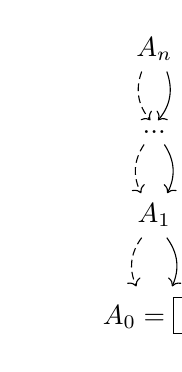
\begin{tikzpicture}
\begin{tikzcd}
    A_n \arrow[d, dashed, bend right] \arrow[d, bend left] \\
    ... \arrow[d, dashed, bend right] \arrow[d, bend left] \\
    A_1 \arrow[d, dashed, bend right] \arrow[d, bend left] \\
    A_0 = \boxed{1}
\end{tikzcd}
\end{tikzpicture}
\end{wrapfigure}

Even more specifically, we define abstract chains as diagrams that have at most one left child and one right child, and if having two children, those two children being equal. We define $\mathcal{D}^{\dagger} = \bigcup_{n \in \mathbb{N}} \mathcal{D}^{\dagger}_n$ the set of all abstract chains, with $\mathcal{D}^{\dagger}_n$ the set of abstract chains of height $n$.


\chapter{Reduction algorithm}

\chapter{Reduction algorithm}

We note that multiple QDDs can be evaluated to the same abstract state. This part will aim to provide an algorithm to decrease the "size" of diagrams while not breaking their evaluation by $\mathcal{E}$. The size of a AAQDD is the number of intervals (counting them with their multiplicity). We would want, from a diagram $D$, to get a diagram $D'$ such that $\text{size}(D) > \text{size}(D')$ and $D \le D'$ (the reduction is smaller in size and might be less precise that the original diagram). More generally, function $g : \mathcal{D}_n \rightarrow \mathcal{D}_n$ is an \textit{global approximation} if
$$\forall D \in \mathcal{D}_n, D \le g(D)$$

Similarly, a function $f : \mathcal{D}_n \times \mathcal{D}_n \rightarrow \mathcal{D}_n$ is a \textit{merge approximation at height $n$} if
$$\begin{cases}
    \forall A \not= B \in \mathcal{D}_n, A \le f(A, B)~\text{and}~B \le f(A, B) \\
    \forall A \in \mathcal{D}_n, f(A, A) = A
\end{cases}
$$

We developed a reduction formula to force the merging of two nodes. This is permitted both thanks to abstract interpretation (to merge without amplitudes being colinear) and the additive nature of diagrams. The cost $\mathcal{C}_f : \mathcal{D}_n \rightarrow \mathbb{R}^+$ of applying a global approximation $f$ to a diagram $D \in \mathcal{D}_n$ is defined by:

$$\mathcal{C}_f(D) = \mathcal{I}(f(D)) - \mathcal{I}(D)$$

\section{Merging theorem}

Let $n \in \mathbb{N}^*$, $N \ge n$, and $f$ be a merge approximation. Moreover let $w : \mathcal{D}_N \rightarrow \mathcal{D}_n \times \mathcal{D}_n$ be a choice function at height $n$ in $\mathcal{D}_N$, meaning that $\forall D, w(D) \in \mathcal{N}_n(D) \times \mathcal{N}_n(D)$. Now we define:

$$\function{f | w}{\mathcal{D}_N}{\mathcal{D}_N}{D}{r_N(B, C, r_N(A, C, D))\quad \text{with}~C = f(w(D))}$$

With $\forall i > 0, r_i : \mathcal{D}_n \times \mathcal{D}_n \times \mathcal{D}_i \rightarrow \mathcal{D}_i$ the replacement function defined by:
$$\begin{cases}
\forall n > i, \forall A, B \in \mathcal{D}_n, \forall D \in \mathcal{D}_i, r_i(A, B, D) = D \\
\forall A, B, D \in \mathcal{D}_n, r_n(A, B, D) = \begin{cases}
B \quad \text{if}~D = A \\
D \quad \text{otherwise}
\end{cases} \\
\forall 1 \le n < i, \forall A, B \in \mathcal{D}_n, \forall \{(\alpha_j, g_j)\}, \{(\beta_k, d_k)\} \in \mathcal{D}_{i-1},\\
\hfill r_i(A, B, (G, D)) = (\{(\alpha_j, r_{i-1}(g_j))\}, \{(\beta_k, r_{i-1}(d_k))\})
\end{cases}
$$

\noindent\underline{\textbf{Merging theorem:}} Let $f$ be a merge approximation at height $n$ and $w$ be a choice function at height $n$ in $\mathcal{D}_N$. $f|w$ is a global approximation in $\mathcal{D}_N$.

\noindent\underline{Proof:} Let $D \in \mathcal{D}_N$, $(A, B) = w(D)$ and $C = f(w(D))$. By ascending induction (in height), it comes that $\forall U, V \in \mathcal{D}_n, U \le V \Rightarrow r_N(U, V, D) \le D$. Meanwhile, $f$ is a merge approximation so $A \le C$, thus $r_N(A, C, D) \le D$.

Proving that $r_N(A, C, D) \le D$ is mostly enough to prove the theorem, because once it is proven we only have let $D' = r_N(A, C, D)$ and use this result on $B$ and $D'$ to conclude that $r_N(B, C, D') \le D'$. The only problem is that we would need $C' = f(w(D'))$ instead of $C$ to reuse the exact same result demonstrated earlier.
\hfill{} $\boxed{}$


\section{One-side case}

To begin, let's consider the simple case where all diagrams only have left children (this case would be useless in practice because it would result in only one interval and zeros). Let's say we want to merge the two diagrams:
\begin{gather*}
A = (\{(\alpha_0, a_0), ..., (\alpha_{l-1}, a_{l-1}), (\beta(A)_0, b_0), ..., (\beta(A)_{n-1}, b_{n-1})\}, \emptyset)\quad \text{and} \\
C = (\{ (\beta(C)_0, b_0), ..., (\beta(C)_{n-1}, b_{n-1}), (\gamma_0, c_0), ..., (\gamma_m, c_{m-1}) \}, \emptyset)
\end{gather*}
\noindent with $\{a_0, ..., a_{l-1}\} \cap \{c_0, ..., c_{m-1}\} = \emptyset$. A graphic representation of our merging formula would be:

\vspace{1.7cm}
\leftskip=200pt
% https://tikzcd.yichuanshen.de/#N4Igdg9gJgpgziAXAbVABwnAlgFyxMJZAJgBoAGAXVJADcBDAGwFcYkQQBfU9TXfQigAsFanSat2XHiAzY8BIgHZRNBizaIO3XvIFEAnKvEapO2XwWCSpAIxj1krQEFpu-ouF2HEzSADCbhZ6nsgArN5qvmYych7WKvZRplpBcVZEAByRJk4gADr5ODAAHjjAALYwAE4A5jCcABTOpAAE-gCUaZb6KOSkxD4pIPQA+uTdIda2A0N5Y8CMALS2nJPxRGSDyXkARuPrGSgAzLM7fvvAYCtr5um9yCLbuX4Axgd3PaERz45vo5UbocHgA2M4vdhjCafKbKcF-SEA5arYGhbK-aJafbQ2JfaxGDHDS7XFEwjYoWz9Ql5d449xHZC2GbU-6A0liGBQeoIFCgABm1QgFSQ-RAOAgSBEEK0zBANEY9F2MEYAAU8exGDA+TgggKhUgZmKJYgItK6HKQAqlar1VpNdrdYLhYgyEakNkzbL5YrlWrYXatTrzHrnac3YgPQitLQLVbfbaQNUsLUABZBmQhyU0cUG0VRsDMRiMb3Wv3ky2Bx36xBSnOIJnnJAFosl+P+isO4NOrPh2yuqMFfJKnD0ZodUYAK1jPpt7ft6f53Zr2eNRjNhSYaBTYyw09LCaTqYXIEzJpXBsN+cLxctM7LRw7x9PprrfcbWkKw9HACFx1PW7O5bzlWzovsathhleLa3vuc6Vl21ZgQaUoDoUtT0BUFRjAA1nubZAfBGZLmC4YqGajR8hUXQAfevSPrGWBgH4UAQMwuyaiB7rnvWJFQTecaAQ+wEIc6HqvmRqH5LAjAjpOeGCXRwlEdWYngZGmLNvxd4Jkpi4qdxtimpJm7bqMu40QeyZppxEYGWufEWXBnbKaJ3HEHmmKDuhmE4fJtGePRIlIGur4eSkmmOQRDo0CmMD0FA7CQExDHJVoUD0HAsUJUF9aGq+-YadekVCZWMVxQlWhJWw8qMcxGVZTZEEGShhXQQJ-mCPRZXxYlBDVZatXsOlmWco1SE8e+EUwfhJXRSAsU9ZVfUpXVI3ZS5Bpka+6nhUV00KQFwHdRV4DLTVqUgMNDU5bYIXGu5k17e1OmlfN5W9cl52rddlCcEAA
\begin{tikzcd}[overlay]
                               &         & {} \arrow[d, "u"]                                                        &         & {} \arrow[d, "v"]                                                       &                                   &                                & {} \arrow[rd, "u"] &                                                                                                                                & {} \arrow[ld, "v"'] &                                &         \\
                               &         & A \arrow[ld] \arrow[d] \arrow[rd, "\beta(A)_j"] \arrow[lld, "\alpha_i"'] &         & C \arrow[lld] \arrow[ld, "\beta(B)_j"] \arrow[d] \arrow[rd, "\gamma_k"] & {} \arrow[rr, "(\text{fm})", Rightarrow] &                                & {}                 & {\text{fm}(A, C)} \arrow[ld] \arrow[d, "\delta_j"] \arrow[rd] \arrow[lld, "\alpha_i"'] \arrow[rrd] \arrow[rrrd, "\gamma_k"] &                     &                                &         \\
a_0 \arrow[r, no head, dashed] & a_{l-1} & b_0 \arrow[r, no head, dashed]                                           & b_{n-1} & c_0 \arrow[r, no head, dashed]                                          & c_{m-1}                           & a_0 \arrow[r, no head, dashed] & a_{l-1}            & b_0 \arrow[r, no head, dashed]                                                                                                 & b_{n-1}             & c_0 \arrow[r, no head, dashed] & c_{m-1}
\end{tikzcd}

\vspace{1.7cm}
\leftskip=0pt

\noindent with $\delta_j = \beta(A)_j \sqcup \beta(B)_j$. More formally, the merging formula would be:
$$\text{fm}(A, C) = (\{(\alpha_0, a_0), ..., (\alpha_{l-1}, a_{l-1}), (\delta_0, b_0), ..., (\delta_{n-1}, b_{n-1}), (\gamma_0, c_0), ..., (\gamma_m, c_{m-1})\}, \emptyset)$$

\section{Fully connected case}


Let's consider another case, where our two nodes $A$ and $B$ have both a common left-descendance and a common right-descendance. We will see later that the general case can always be reduced to this case. The abstract amplitude on the link between two nodes is $\text{ampl}(u, v)$, for example $\text{ampl}(A, l_0)$ or $\text{ampl}(B, l_0)$. Additionally, let $X = \{l_0, ..., l_{k-1}, r_0, ..., r_{m-1}\}$.

\vspace{1.7cm}
\leftskip=200pt
% https://tikzcd.yichuanshen.de/#N4Igdg9gJgpgziAXAbVABwnAlgFyxMJZAJgBoAGAXVJADcBDAGwFcYkQBBEAX1PU1z5CKACwVqdJq3YAhHnxAZseAkXKliEhizaIQjAPrl5-ZUKJlNNbdL2HgYALQBGbicUCVw5GKuSd7ABORu5KgqooAGwaWlK6IMHAALYubrym4d4A7DHWceyGxukeZhHIAJy5-rb6Bg6poZ7mKM7OVTbxwUUKYV5EzgDM7fl6iSmujaXezupUeQF6AMIABAC8ywA6GzgwAB44wABmSdwAFBykyzIAlJOZRNHOsQsgd30oABykT-M1PBIwKAAc3gRFAh0CECSSHUIBwECQZH0WDA8Sg9DgAAtAe4IVCYTR4UghsjUex0ViccU8dDEEiiYgSYwUWiIDgdlAQDRsfROXpIGTqZDaW04Qi6TRmWS9BTsZyhfjEKKGUyWeSMXLccKCWKkCIFSLCeL9QoaTqGQBWA16o1IC3cmC89gCtiStUytkcrWK5Xiq2m7WIaK6xA5Ums9k4h1O-kENjWxBfEOVEA8vngONc8Pkz1UgM+2EMsNStEavPgwMzW2JhNV5O131IZxIks55gAI0YrtTjr5YGYjEYhPoWEYzszv3iWx2+2Ap2O1zS+ZFhfFwdbMrL8so3CAA
\begin{tikzcd}[overlay]
                                &  & A \arrow[lldd, dashed] \arrow[dd, dashed] \arrow[rrdd] \arrow[rrrrdd] &  & B \arrow[lllldd, dashed] \arrow[lldd, dashed] \arrow[dd] \arrow[rrdd] &  &                                          &                                 &    &         & {C = \text{fm}(A, B)} \arrow[ldd, dashed] \arrow[rdd] \arrow[rrrdd] \arrow[llldd, dashed] &                                 &  &         \\
                                &  &                                                                       &  &                                                                       &  & {} \arrow[rr, "\text{(fm)}", Rightarrow] &                                 & {} &         &                                                                                           &                                 &  &         \\
l_0 \arrow[rr, no head, dotted] &  & l_{k-1}                                                               &  & r_0 \arrow[rr, no head, dotted]                                       &  & r_{m-1}                                  & l_0 \arrow[rr, no head, dotted] &    & l_{k-1} &                                                                                           & r_0 \arrow[rr, no head, dotted] &  & r_{m-1}
\end{tikzcd}

\vspace{1.7cm}
\leftskip=0pt

Where the new abstract amplitudes are defined by the following formula:

$$\forall x \in X, \text{ampl}(C, x) = \text{ampl}(A, x) \sqcup \text{ampl}(B, x)$$

\noindent\underline{\textbf{Proof:}} Let $f : \mathcal{D}_n \times \mathcal{D}_n \rightarrow \mathcal{D}_n$ be our diagram transofrmation.
Let $\alpha_0, \alpha_1, \beta_0, \beta_1 \in \mathcal{A}_0$ such that $\alpha_0 \subset \beta_0$ and $\alpha_1 \subset \beta_1$.
\begin{align*}
&\min(\min \RE(\beta_0), \min \RE(\beta_1)) \le \min(\min \RE(\alpha_0), \min \RE(\alpha_1)) & \text{and} \\
&\max(\max \RE(\beta_0), \max \RE(\beta_1)) \ge \max(\max \RE(\alpha_0), \max \RE(\alpha_1))&
\end{align*}

\noindent thus $\RE(\alpha_0 \sqcup \alpha_1) \subset \RE(\beta_0 \sqcup \beta_1)$. The same goes for imaginary parts, hence $\alpha_0 \sqcup \alpha_1 \subset \beta_0 \sqcup \beta_1$.
With a very similar proof, we can show that $\alpha_0 + \alpha_1 \subset \beta_0 + \beta_1$.

From there it comes that $\forall x \in X, \text{ampl}(A, x) \subset \text{ampl}(C, x)$ and $\forall x \in X, \text{ampl}(B, x) \subset \text{ampl}(C, x)$, and inductively:
\begin{align*}
\displaystyle\sum_{l \in \{l_0, ..., l_{k-1}\}} \text{ampl}(A, l) * l \subset &\displaystyle\sum_{l \in \{l_0, ..., l_{k-1}\}} \text{ampl}(C, l) * l\quad\quad \text{and} \\
\displaystyle\sum_{r \in \{r_0, ..., r_{m-1}\}} \text{ampl}(A, r) * r\subset &\displaystyle\sum_{r \in \{r_0, ..., r_{m-1}\}} \text{ampl}(C, r) * r
\end{align*}

We now have $A \le C$, and since $A$ and $B$ are interchangeable, $B \le C$. Consequently, $f$ is a merge approximation and according to the merging theorem, a global approximation can be derived from it.
\hfill{} $\boxed{}$

\section{Error estimation}

Let $A, C \in \mathcal{D}_n$. We would like to define a scale $\delta : \mathcal{D}_n \rightarrow X$ with $(X, \prec)$ a partially ordered set, that we would be able to compute in polynomial time and space (i.e. in $O(n^p)$ for a certain $p \in \mathbb{N}$), such that if $A \le C$, $\delta(A) \prec \delta(C)$. Let $X = \mathbb{R}^+ \times \mathcal{A}_0$ and $\delta(A) = (|A|, [A])$ be inductively defined by:
$$\delta(\boxed{1}) = (1, [1, 1])$$
$$\forall a, b \in \mathcal{A}_0, \delta(\{(a, \boxed{1})\}, \{(b, \boxed{1})\}) = $$
$$\forall G, D \in \mathscr{P}_f(\mathcal{A}_0 \times \mathcal{D}_n), |(G, D)|
= \max\left( \left|\sum_{(l, L) \in G} l |L| \right|, \left|\sum_{(r, R) \in D} r |R| \right|\right)$$
$$\forall G, D \in \mathscr{P}_f(\mathcal{A}_0 \times \mathcal{D}_n), [(G, D)]
= \left(\sum_{(l, L) \in G} l |L| [L] \right) \bigsqcup \left(\sum_{(r, R) \in D} r |R| [R]\right)$$

\noindent\underline{\textbf{Proof:}} Let for $n \ge 0$ the property
$$(\Delta_n)\quad : \quad \forall A, B \in \mathcal{D}_n, A \le B \Rightarrow \delta(A) \prec \delta(B)$$

\noindent\boxed{n = 0} The only zero-height diagram is $\boxed{1}$, the result is trivial.

\noindent\boxed{n = 1} Let $A, B \in \mathcal{D}_1$.

\begin{center}
% https://tikzcd.yichuanshen.de/#N4Igdg9gJgpgziAXAbVABwnAlgFyxMJZABgBpiBdUkANwEMAbAVxiRAEEQBfU9TXfIRQAmclVqMWbAELdeIDNjwEiZAIzj6zVohAAdPQCMIADxhRgarnL5LBRURupapug8bMWr3ceYDm8ESgAGYAThAAtkhkIDgQSKIS2mx0APoMAH4ZINQMdIYwDAAK-MpCIKFYfgAWODkgDFhgOiBQdHDV5vUFYFBIALQALACcPCHhUYgxcQnOki1ZaaH1eQXFpfa6DDDBddQ9fYgjYyBhkUhq1DOIAMxzybqG6Vkr+YUldiq6lTV7DU0tNodLr7GC9AbHeRnSaXWLxW73VwgLJPZa5N7rT7lba7bpgw7HChcIA
\begin{tikzcd}
A \arrow[d, "a_l~~"', dashed, bend right=49] \arrow[d, "~~a_r", bend left=49] &  & B \arrow[d, "b_l~~"', dashed, bend right=49] \arrow[d, "~~b_r", bend left=49] \\
\boxed{1}                                                                     &  & \boxed{1}
\end{tikzcd}
\end{center}

Suppose that $A \le B$, then $a_l \le b_l$ and $a_r \le b_r$, hence $a_l [\boxed{1}] \sqcup a_r [\boxed{1}] = a_l + a_r \le b_l + b_r$, and then $\delta(A) \prec \delta(B)$, so $(\Delta_1)$ is true.

\noindent\boxed{n > 1} Let $n > 1$ such that $(\Delta_{n-1})$ is true. Let $A, B \in \mathcal{D}_n$ such that $A \le B$.

% https://tikzcd.yichuanshen.de/#N4Igdg9gJgpgziAXAbVABwnAlgFyxMJZAJgBoAGAXVJADcBDAGwFcYkQBBEAX1PU1z5CKAKwVqdJq3YAhHnxAZseAkXKkAjBIYs2iEABkA+hvn9lQohs3apew0cK9zg1SjJaaO6foBKJs0UBFWFkAGYbLzt2fwBbQKVXUIAWSMlddmNTZyCLN2QxT3SfBycFRJCiADY073t-bPLgyxQAdlrovyN47gkYKABzeCJQADMAJwh4xHUQHAgkCOK9MGZGRhpGegAjGEYABWa3EEYYUZwQTawweyh6OAALfsCJqaRZ+aRU5aRV9c2dntDnlhCczhccq9ph8FogxD9EH8NidAQcjqDTucXpNoTRPogyAikQDdmiQexMRcrjd2HdHs9ITikNY5rCakS1sitqTgUkKeDLidrrd7k8oNi3ogWfj2hz-iieej+VjqSL6eLGZLpbCABxRDKIzkkoFK-SUiXTbVIACc+p8xIVJvJZoFmumhPxSzqvyNjrJfJdKpAT3o4v0kBpqtpEBwOAZCihXzxsPh3sN8u5ToDYKDIbD4AIbCj+igMbjGoTTMQ7JldpWvsz-sqgapwZgofYEaLQppJbL8bGVb1rJtdZ9GdRvObOdbec7hcFjGF0djDMo3CAA
\begin{tikzcd}
                               &     & A \arrow[ld, dashed] \arrow[d] \arrow[rd] \arrow[lld, dashed] &     &                                & B \arrow[ld, dashed] \arrow[d, dashed] \arrow[rd] \arrow[rrd] &                                &     \\
L_1 \arrow[r, no head, dotted] & L_n & R_1 \arrow[r, no head, dotted]                                & R_m & L_1 \arrow[r, no head, dotted] & L_n                                                           & R_1 \arrow[r, no head, dotted] & R_m
\end{tikzcd}

Let $a_j = \text{ampl}(j, A)$ and $b_j = \text{ampl}(j, B)$. We know that $A \le B$ so:
$$\sum_j a_j \mathcal{E}(j) \le \sum_j b_j \mathcal{E}(j)$$

We would like to prove that:
$$|A \le |B|, ~\text{i.e.}~ \max()$$


\end{document}
